\section{Implementierung analoger Regler}


\subsection{Struktur allgemeiner Frequenzgang}


\subsection{Grundschaltungen mit OpAmps}

\subsubsection{Summator}

\begin{minipage}[c]{0.48\columnwidth}
    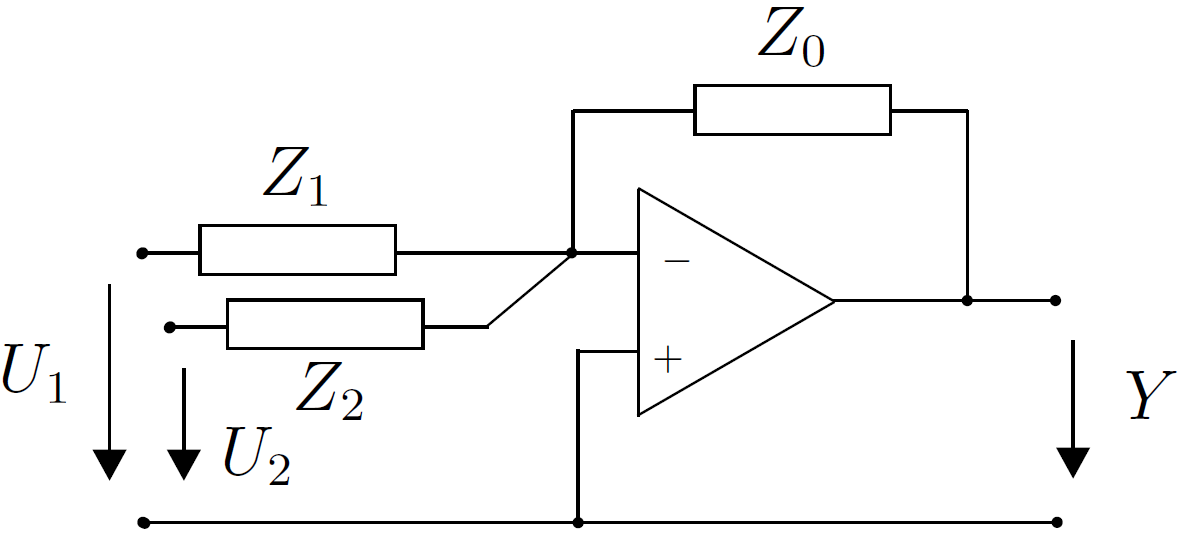
\includegraphics[width=\columnwidth]{images/opamp_grundschaltung_2_eingaenge.png}
\end{minipage}
\hfill
\begin{minipage}[c]{0.48\columnwidth}
    
\end{minipage}


\subsubsection{Integrierer}

\begin{minipage}[c]{0.48\columnwidth}
    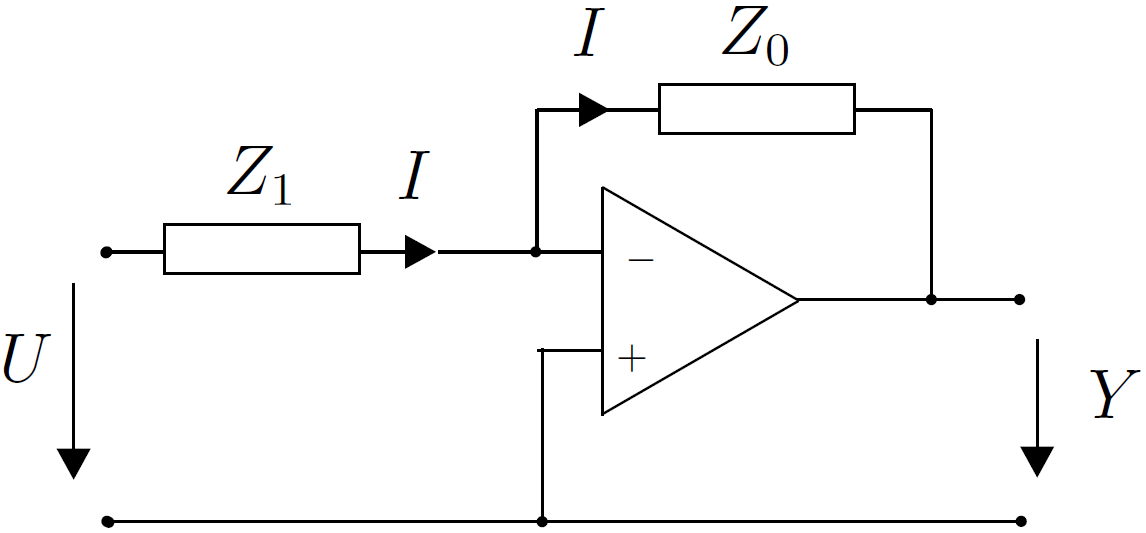
\includegraphics[width=\columnwidth]{images/opamp_grundschaltung_1_eingang.png}
\end{minipage}
\hfill
\begin{minipage}[c]{0.48\columnwidth}
    
\end{minipage}


\subsubsection{P-Glied (passiv)}

\begin{minipage}[c]{0.48\columnwidth}
    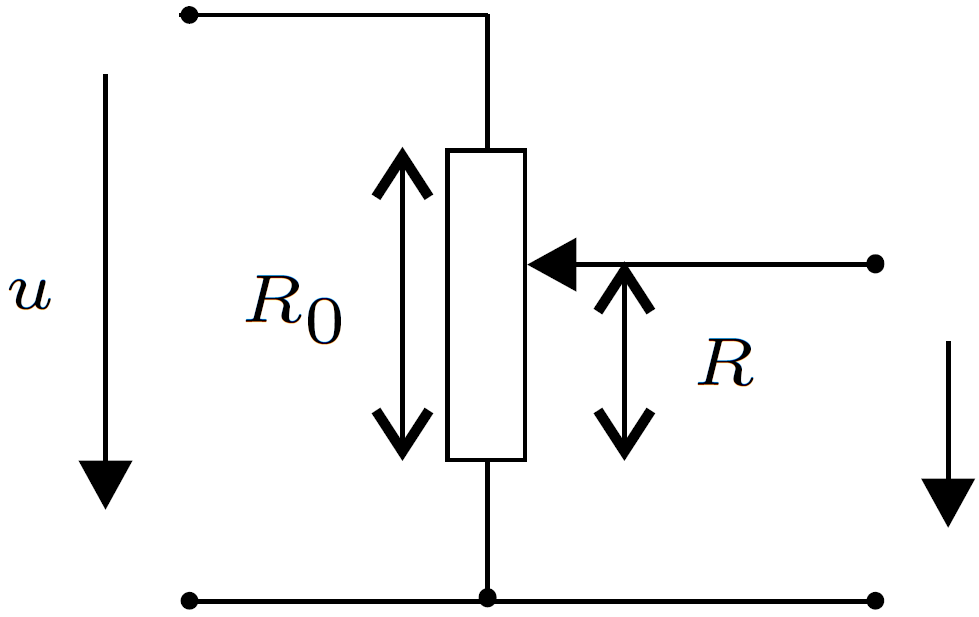
\includegraphics[width=\columnwidth]{images/spannungsteiler.png}
\end{minipage}
\hfill
\begin{minipage}[c]{0.48\columnwidth}
    
\end{minipage}




\subsection{Varianten analoger PID-Schaltungen}

\subsubsection{Variante 1 (gemischt)}

\begin{minipage}[c]{0.48\columnwidth}
    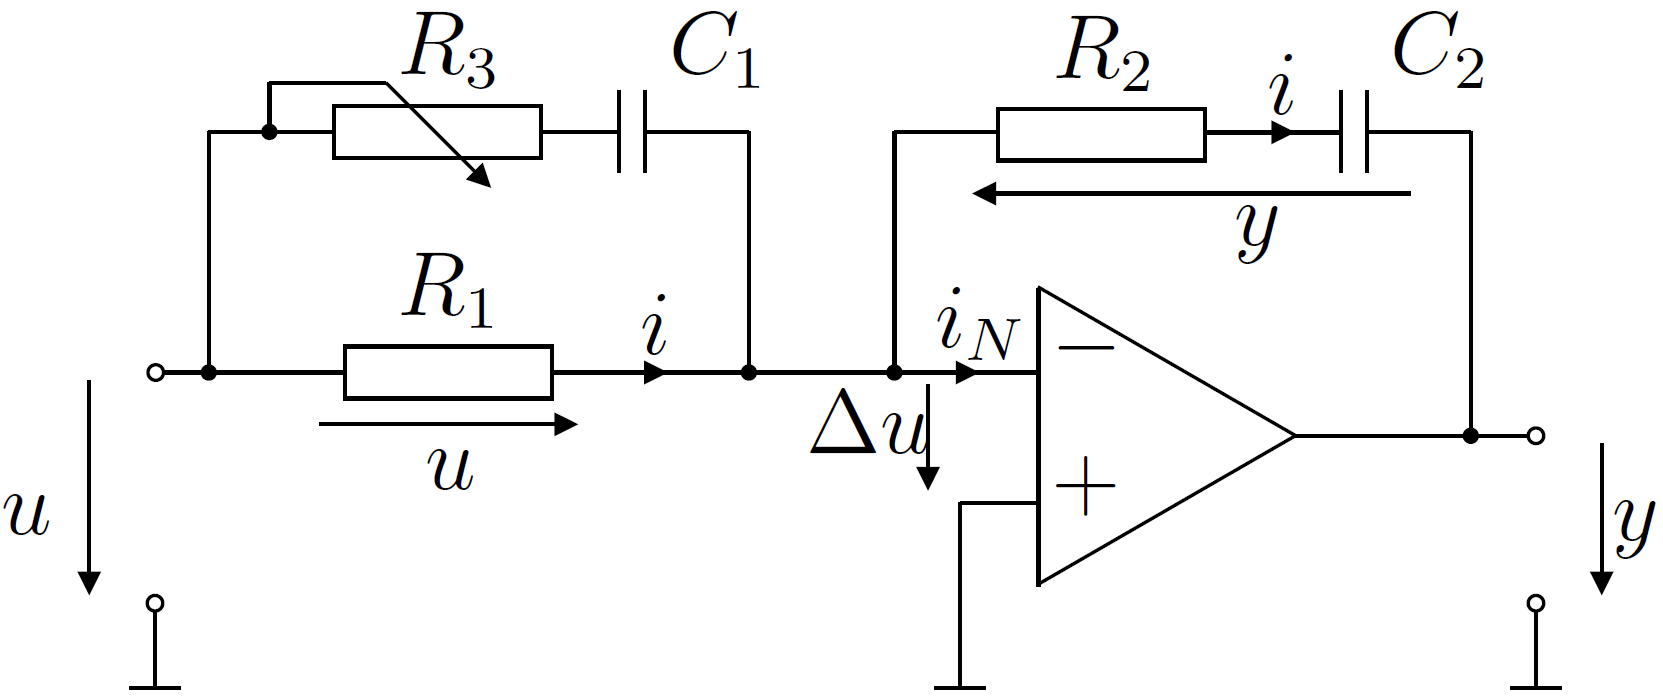
\includegraphics[width=\columnwidth]{images/realisierung_pid-regler_variante_1.png}
\end{minipage}
\hfill
\begin{minipage}[c]{0.48\columnwidth}
    
\end{minipage}


\subsubsection{Variante 2 (Parallelform)}

\begin{minipage}[c]{0.48\columnwidth}
    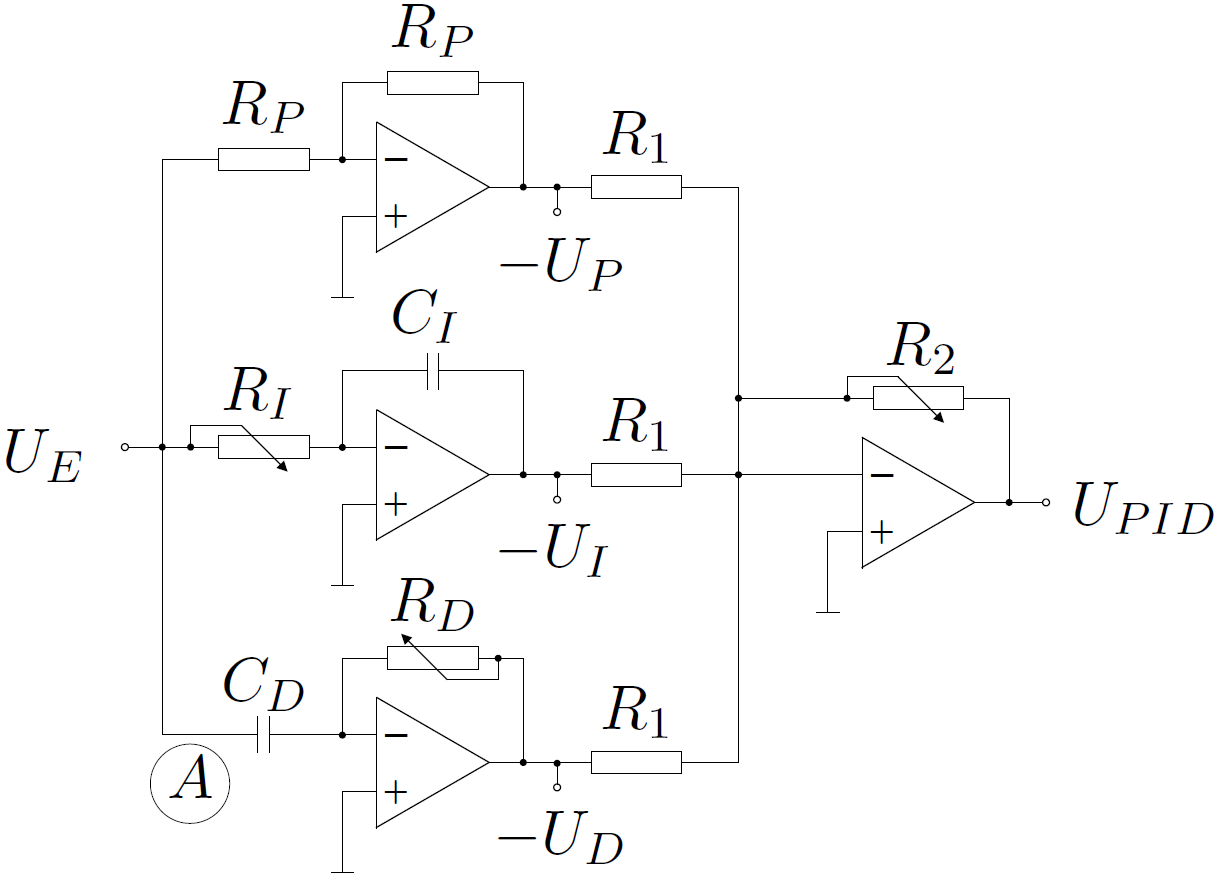
\includegraphics[width=\columnwidth]{images/realisierung_pid-regler_variante_2.png}
\end{minipage}
\hfill
\begin{minipage}[c]{0.48\columnwidth}
    
\end{minipage}